\chapter{Non-Dimesional Analysis}
One of the ways we can analyse the stockpile model,
\begin{equation}
\rho c \frac{\partial T}{\partial t}=\nabla \cdot \left(k\nabla T\right) +Q(T), \label{base2}
\end{equation}
stated in section \ref{Sec:stockpile}, is through non-dimensional analysis. In this technique we scale the dimensional variables, $x$, $t$ and $T$ using the constants that appear in the equations. This analysis allows us to determine some of the general features of the stockpiles. This analysis has been used to determine a relationship for the critical length of a stockpile, dependant upon the reaction kinetics. Within this chapter we will analyse, through non-dimensional analysis the effects that periodic boundary condition can have on stockpile ignition and also the effects of a hotspot within the stockpile for subcritical stockpile.\\

Considering a one-dimensional stockpile, of length $L$, with a first order Arrhenious reaction rate, we can use the scalings,
\begin{align*}
x^*&=\frac{x}{L},\\
t^*&= \frac{\alpha}{L^2}t, \\
u&=\frac{E}{RT_a^2}\left(T-T_a\right),
\end{align*} 
to reduce the equation to the non-dimensioanal form,
\begin{equation}
\frac{\partial u}{\partial t^*}=\frac{\partial^2 u}{\partial {x^*}^2}+\delta\exp\left(\frac{u}{1+\varepsilon u}\right), \label{eq:non-dim}
\end{equation}
where,
where $\varepsilon=T_a R/E$ and $$\delta=L_y^2\frac{Q\rho A}{k}\exp\left(\frac{-E}{RT_a}\right)\frac{E}{R T_a^2}.$$ The parameter $\delta$ is the Frank-Kamanetskii (FK) parameter. Using the Dirichlet boundary condition, $T=Ta$, then we obtain the non-dimensional boundary condition $u=0$. The domain of our scaled equation is $x^*\in [0,1]$. With this formulation we often have $\varepsilon \ll 1$ so we consider $\varepsilon=0$. In this case we have a critical Frank-Kamanetskii parameter such that if $\delta>\delta_{\text{cr}}$ then the stockpile will ignite, and if $\delta<\delta_{\text{cr}} $ then the stockpile will not ignite and is considered subcritical.\\

We can extend this non-dimensionalisation to higher spatial dimensions. If we consider three dimensions, $(x,y,z)$, then by scaling everything by the height, $L_y$, then Equation \ref{base2}, becomes,
\begin{equation}
\frac{\partial u}{\partial t^*}=\frac{\partial^2 u}{\partial {x^*}^2}+\frac{\partial^2 u}{\partial {y^*}^2}+\frac{\partial^2 u}{\partial {z^*}^2}+\delta\exp\left(\frac{u}{1+\varepsilon u}\right),
\end{equation}
on the domain $[0,L_x/L_y]\times[0,1]\times[0,L_z/L_y]$. We scale each spatial dimension by the same length since we maintain the laplacian in the equation. In this case the results are still dependant upon the shape of the domain but generally we will consider nice shapes where the lengths have certain nice ratios. From here we drop the $*$ from the dimensionless variables.\\

We need to define what we mean by ignition. In the theoretical case with $\varepsilon=0$, there is a point where there are no stable steady state solutions, and heating continues indefinitely \cite{bowes}. We can then state that supercritical stockpiles are those that will continue heating indefinitely and subcritical are those that do not. This phenomena cannot be determined numerically as we are restricted to finite times and temperatures. This asks the questions how can we define ignition in a practical sense. Within our model there are two things to consider: How hot does the stockpile need to get to to categorise the stockpile as supercritical, and how much time do we allow for the stockpile to reach this state. The answers to these are going to depend on the context of the problem that is being addressed. \\

For our context we generally consider ignition times of approximately one year. For the purposes of our analysis we will consider ignition occouring when the maximum non-dimensional temperature exceeds 100, $u_{\text{max}}=100$. Using the parameters used in a paper we published \cite{Berry19}, this equates to a temperature of roughly $800^oC$. The parameters used here are very similar to those we use in this thesis and as such the critical temperature is roughly $800^oC$. If we were to use a point estimate of $E=10^4.637$ for the experimental data, this would correspond to a critical temperature of $1600^oC$ which would be excessive. This highlights the need for these considerations to be made when applying the non-dimensional results to physical problems. When performing Nonidimensional analysis of the equations we are able to deduce relationships between certain parameters. 


\section{Periodic Boundary Conditions}
In the stockpile literature the boundary conditions do not depend upon time. In practicality the large stockpiles are left outside and subject to seasonal and dirunal variations in the ambient temperature. We only consider seasonal temperature variations within the scope of this thesis. We model the seasonal temperature variations using a sine function. The boundary condition becomes,
\begin{equation}
T=T_a+T_o\sin\left(\frac{2\pi t}{\omega_Y}+\phi\right), \label{eq:PBC_D}
\end{equation}
where $T_a$ is the average ambient temperature variation, $T_o$ is the maximum temperature oscillation, $\omega_Y$ is the oscillation period which for seasonal temperature variations is one year, and $\phi$ is a phase shift. After non=dimensionalising the boundary contition we obtain,
\begin{equation}
u=u_o \sin\left(\frac{2\pi t}{\omega}+\phi \right),
\end{equation} 
where $u_o=\left(E/RT_a^2\right)T_o,$ and $\omega=\alpha \omega_Y/L_y^2.$ The phase shift parameter $\phi$ allows us to control when during the year the stockpiles are constructed. When $\phi=0$, this would be indicative of a stockpile constructed in spring, whilst at $\phi=\pi/2$, this would be during summer when the ambient temperature is at its maximum. This is a very simple way to model the oscillations which also allows us to examine the relationship and effect on stockpile ignition.\\

When we extend this to higher dimensions we don't have all sides exposed to the ambient air. The base of the stockpile requires a seperate condition. For simplicity we assume that no heat is exchanged at this boundary, that is $\partial T/\partial y =0$. When we have this condition we are able to reflect around the plane $y=0$, which means we can use results where the boundary has the same condition.
 
\subsection{Dirichlet Boundary Condition}
Initially we consider a simple dirichlet boundary condition for two specific stockpile geometries, $L_x=2L_y$ and $L_x=\infty$. For the case where $L_x=2L_y$, the reflective condition prescribed at the boundary $y=0$ means that we can instead solve the problem on the square with non-dimensional length 2. This solution restricted to the domain $(0,2)\times (0,1)$ will solve our equation. For the approximation $\varepsilon=0$ and Dirichlet boundary conditions, the critical value is $\delta_{cr}=1.7$ \cite{bowes}. For $L_x \gg L_y$ we approximate the model by a one-dimensional model without diffusion in the $x$ direction. For the approximation $\varepsilon=0$ and static boundary condition the critical value is $\delta_{cr}=0.88$ \cite{bowes}. The value obtained from our simulations, displayed in Table \ref{1ddelt} equals the value stated by Bowes \cite{bowes} to the given number of significant figures.\\ 
\begin{table}[h!]
\caption{The critical Frank-Kamenetskii parameter, $\delta_{cr}$, in a one dimensional stockpile for different cut-off times with $u_o=0.637$, $\omega=0.3$ and $\phi=0$ for the cases with oscillations.}
\centering
\begin{tabular}{|c|c|c|c|c|c|}
\hline
$\varepsilon$ & Oscillations &$t_f=0.3$& $t_f=1$ & $t_f=10$ & $t_f=100$ \\ \hline
0 & no & 3.701 & 1.582 & 0.899 & 0.877 \\ \hline
0 & yes & 3.428 & 1.537 & 0.895 & 0.875 \\ \hline
0.027 & no & 3.910 & 1.658 & 0.927 & 0.904 \\ \hline
0.027 & yes & 3.639 & 1.612 & 0.924 & 0.901 \\ \hline
\end{tabular}
\label{1ddelt}
\end{table}
Table \ref{1ddelt} suggests that for the larger cut-off times ($t_f=10,100$) the dynamic boundary condition does not have a significant influence on the critical FK parameter with a slight reduction observed, when the oscillations are added. However, there is a significant difference in the ignition times.
For the case where $\varepsilon=0$, $\delta=0.89$, the ignition times are $\tig=14.00$ and $\tig=12.04$, for the dynamic and static boundary conditions respectively. Similarly for $\varepsilon=0.027$, $\delta=0.92$ and the static boundary condition, $\tig=12.40$ whilst with the dynamic boundary condition, $\tig=11.67$. This indicates that for a given stockpile the ignition time is different once the dynamic boundary condition is applied. \\ 
\begin{table}[h!]
\caption{The critical FK parameter $\delta_{cr}$ for a two-dimensional rectangular domain with $u_o=0.637$, $\omega=0.3$ and $\phi=0$.}
\centering
\begin{tabular}{|c|c|c|c|c|}
\hline
$\varepsilon$ & Oscillations & $t_f=0.3$ & $t_f=1$ & $t_f=10$ \\ \hline
0 & no & 4.072 & 2.20 & 1.71  \\ \hline
0 & yes & 3.615 & 2.14 & 1.69  \\ \hline
0.027 & no & 4.294 & 2.3 & 1.76  \\ \hline
0.027 & yes & 3.843 & 2.23 & 1.75  \\ \hline
\end{tabular}
\label{2ddelt}
\end{table}  
In two dimensions, the effects of the dynamic boundary condition are more prominent than with the static boundary condition. For the $\varepsilon=0$ case, the oscillations cause stockpiles to ignite that are \textit{subcritical} when considering a static boundary condition. The one-dimensional stockpiles have a lower critical value so one would expect as we increase the length, $L_x$, of the two-dimensional stockpile with fixed height, $L_y$, then this will decrease the critical parameter. This relationship is displayed in Figure \ref{ratio}.
\begin{figure}[h!]
\centering
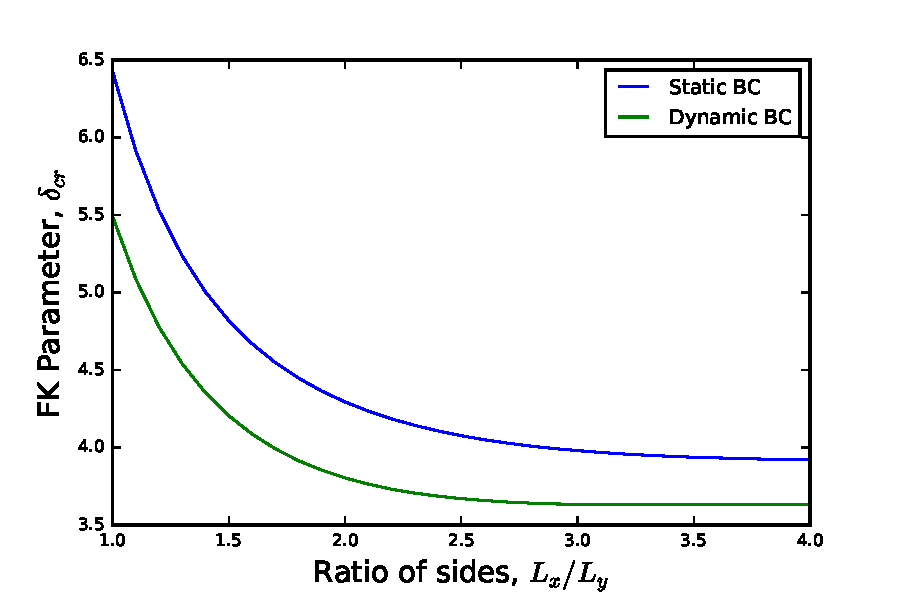
\includegraphics[scale=0.8]{figures/NDA/PBC/deltavslength_both.pdf} 
\caption{The critical FK variable $\delta$ for ignition to occur within a year, as the ratio of side length to height is increased with $\epsilon=0.027$ and $\phi=0$.}
\label{ratio}
\end{figure}
For the static boundary condition, the critical value of the FK parameter approaches that calculated for the one dimensional model. \\
So far our analysis has assumed the stockpiles are constructed at a specific time of year, specifically spring, $\phi=0$. By setting $t_f=0.3$, Figure \ref{phi} indicates which stockpiles will ignite within a year. Certain stockpiles constructed in spring will ignite whilst identical ones constructed in Autumn will not.\\ 
\begin{figure}[h!]
\centering
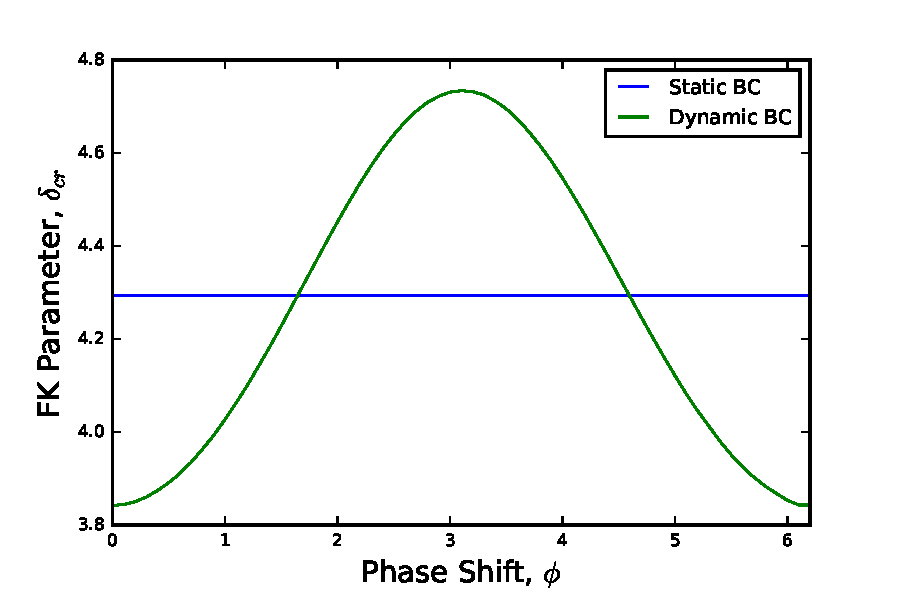
\includegraphics[scale=0.8]{figures/NDA/PBC/phaseshift.pdf} 
\caption{The effects of changing the stockpile construction time ($\phi$) on the critical FK parameter, $\delta$, for stockpile ignition within a year ($t_f=0.3$).}
\label{phi}
\end{figure}
\begin{figure}[h!]
\centering
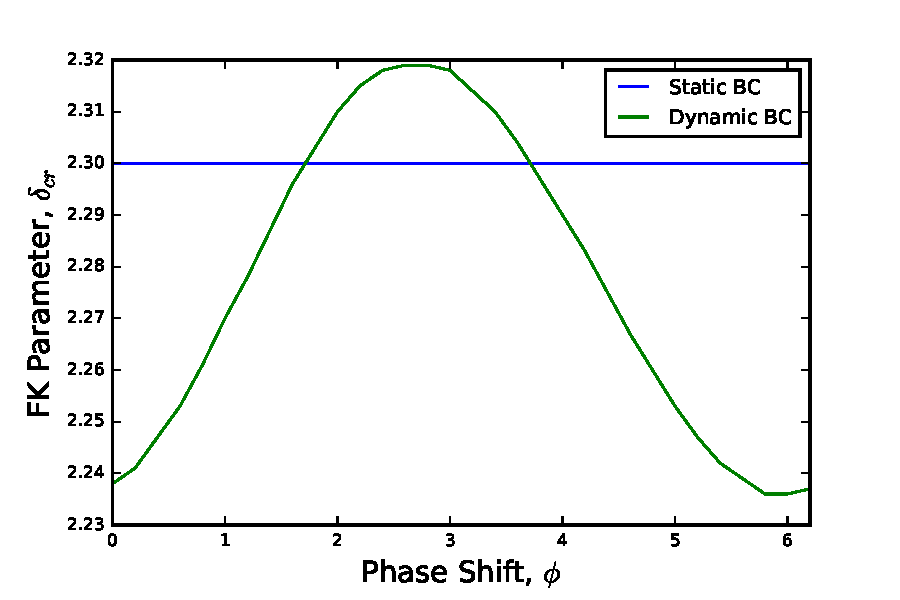
\includegraphics[scale=0.8]{figures/NDA/PBC/phaseshift2.pdf} 
\caption{The effects of changing the initial construction time ($\phi$) on the value of the critical FK parameter, $\delta$, for a final time, $t_f=1$, corresponding to just over a three year period.}
\label{phi2}
\end{figure}
The final time is increased to $t_f=1$. The critical Frank-Kamanetskii parameter becomes less sensitive to the construction date. Another key observation is that when $t_f=1$ there are more starting points where the critical parameter is lower than the static boundary condition. Figure \ref{phi2} shows a shift in the oscillation peak towards $\phi=0$. \\
We now consider the ignition times as the FK parameter ($\delta$) is varied.
\begin{figure}[h!]
\centering
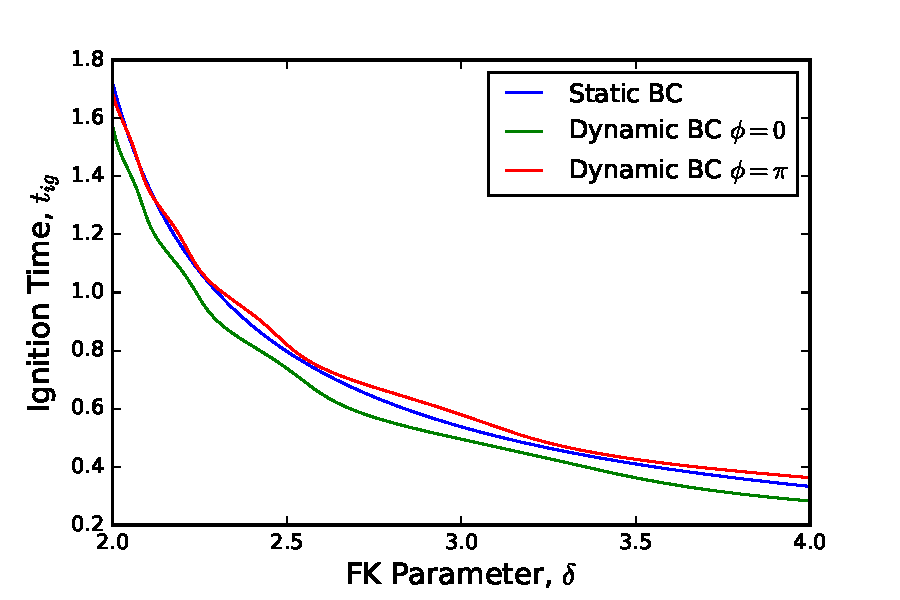
\includegraphics[scale=0.8]{figures/NDA/PBC/ignitontimes.pdf}
\caption{The ignition times as the Frank-Kamanetskii parameter, $\delta$, is varied.}
\label{ignition}
\end{figure} 
Figure \ref{ignition} compares the ignition times for the static boundary condition with the dynamic boundary condition. Stockpiles constructed in spring, $\phi=0$, are plotted along with stockpiles constructed half a year later, $\phi=\pi$. For the larger values of the FK parameter, there is a distinct difference between the ignition times in each case. For smaller values of the FK parameter the ignition times for stockpiles constructed later ($\phi=\pi$) are lower than those with the static boundary condition. This indicates that as we consider longer periods of time the dynamic boundary condition reduces the ignition times. This Figure suggests that there will exist some time such that, regardless of when the stockpile is built, the effect of the dynamic boundary condition will cause the stockpile to ignite earlier than is the case for the static boundary condition.\\

\subsection{Newtonian Cooling Boundary Conditions}
The alternative to using a dirichlet boundary condition is to apply a convective heat transfer condtion. We use the same boundary condition defined in section \ref{Sec:models:BC}, with the ambient temperature following the same oscillations in equation \ref{eq:PBC_D}.
 
\section{Hotspot Ignition}
One of the theories to induce ignition within large stockpiles is to take a portion of material from a supercritical stockpile and add this to a stockpile that is subcritical. From a theoretical basis, in the approximation $\varepsilon=0$, if the temperature within the stockpile is high enough, then the reaction can continue out of control and the stockpile can become supercritical even for FK parameters less than the critical parameter. Since this is a possibility we seek to identify some of the conditions that leads to ignition occurring.\\
We introduce the hotspot by changing the initial temperature distribution. Our initial considerations is a uniform initial condition equal to that of the ambient temperature, ie, $u=0$. We introduce the hotspot by changing the initial condition to,
\begin{equation}
u=u_h\left(H(x-l-w/2)-H(x-l+w/2)\right),
\end{equation} 
where $u_h$ is the dimensionless hotspot temperature, $l$ is the centre location of the hotspot and $w$ is the width of the hotspot, generally expressed in terms of the ratio of hotspot to stockpile size. This formulation allows us to control the location, size and Temperature of the hotspot. We can obtain the nondimensional temperature using the equation,
\begin{equation}
u_h=\frac{E}{RT_a^2}\left(T_h-T_a\right),
\end{equation} 
where $T_h$ is the temperature of the hotspot.

\subsection{One-Dimensional Stockpiles}
To begin our analysis on stockpiles we consider a one-dimensional pile. These piles are the simplest and most computationally efficient to solve. This allows us to examine the dependencies efficiently and then we can generalise these to higher dimension stockpiles. The first relationship we explore is for a fixed size hotspot, how hot does this hotspot need to be in order to cause a subcritical stockpile to ignite. Figure \ref{fig:hot:delta1} displays this relation and indicates what we would expect that as we decrease the Frank-Kamanetskii parameter then we require a hotter hotspot to cause ignition.\\

\begin{figure}[h!]
\centering
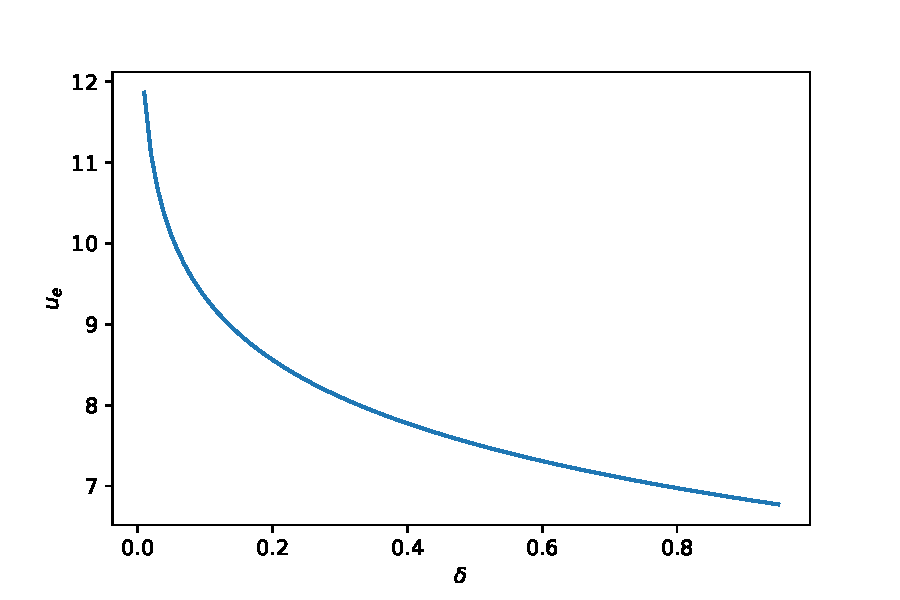
\includegraphics[width=\linewidth]{figures/NDA/Hotspot/delta1.pdf}  
\caption{The temperature required for subcritical stockpile to ignite.}
\label{fig:hot:delta1}
\end{figure} 

Figure \ref{fig:hot:delta1} uses a hotspot that is 10\% of the size of the stockpile and located on the edge. It is worth investigation what occurs when we change these parameters. Figure \ref{fig:hot:size_loc} displays these results. We find that the size of the hotspot has a significant impact on the critical temperature. Figure \ref{fig:hot:size} also indicates that if the whole stockpile is heated initially to a point equivilant to $40^oC$ with our parameters, then this would be enough to get the stockpile to ignite. The location of the hotspot within the stockpile does not have a large impact on the necessary hotspot temperature. We observe that hotspots near the boundary require a slightly higher temerature and attribute this to the cooling that is occuring at the boundary.\\

\begin{figure}[h!]
\centering
\begin{subfigure}{.5\textwidth}
  \centering
  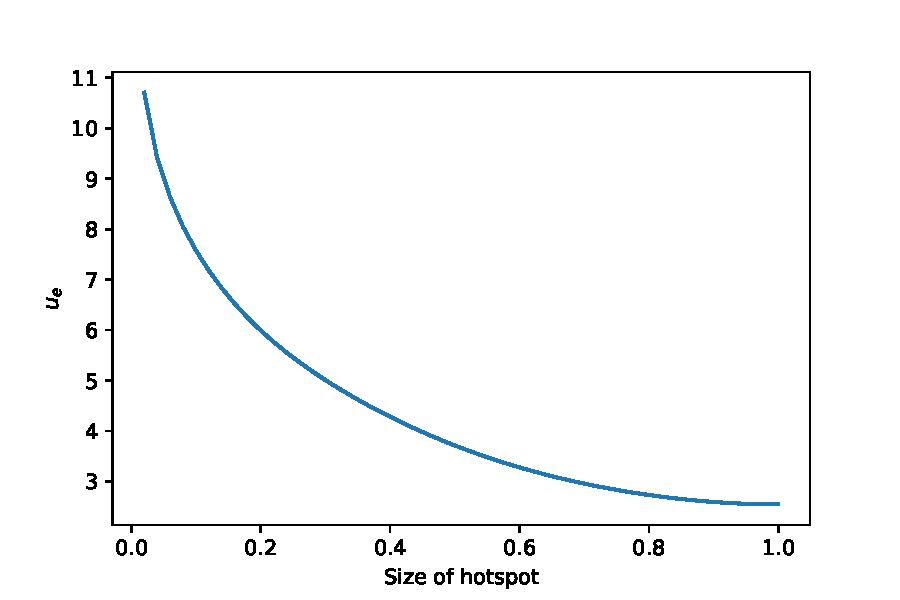
\includegraphics[width=\linewidth]{figures/NDA/Hotspot/size1.pdf}  
  \caption{Hotspot temperature required for different size hotspots.}
  \label{fig:hot:size}
\end{subfigure}%
\begin{subfigure}{.5\textwidth}
  \centering
  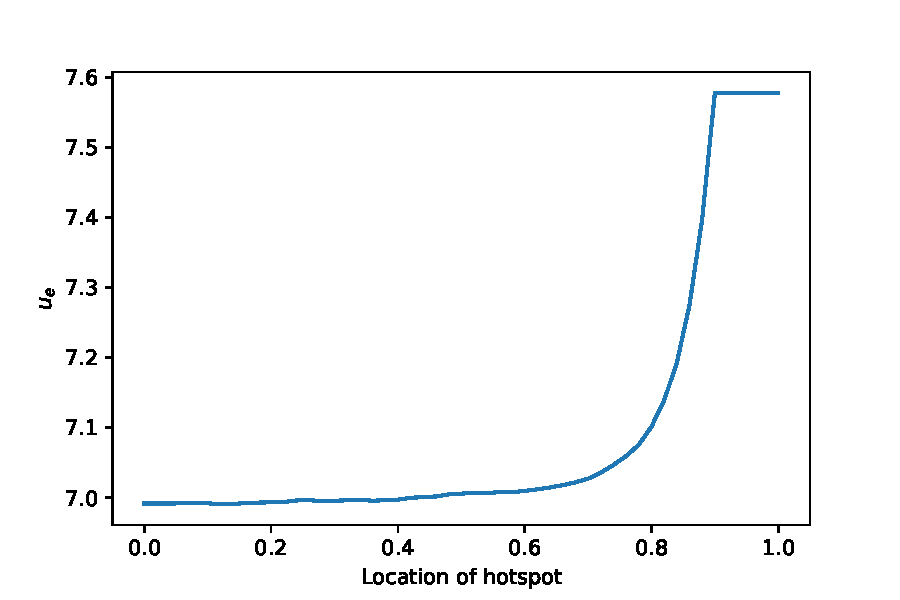
\includegraphics[width=\linewidth]{figures/NDA/Hotspot/Location1.pdf}
  \caption{Hotspot temperature for different hotspot locations}
  \label{fig:hot:loc}
\end{subfigure}
\label{fig:hot:size_loc}
\caption{The critical temperatures needed for different hotspots in order to cause ignition of subcritical stockpiles.}
\end{figure}

In the previous section we determined that periodic boundary conditions had an impact on the the critical delta parameter. It would then be useful to know if this has an impact on the critical hotspot temperature required for ignition. Figure \ref{fig:hot:phi} indicates that there is minimal effect of the time of year these hotspots are added to the piles. In our application the critical temperature varies by less than a degree. We can compare the to the critical hotspot temperature without periodic boundary conditions, which is $7.526$, and this indicates that we get an increase in the critical temperature required, this is not a significant difference. \\

\begin{figure}[h!]
\centering
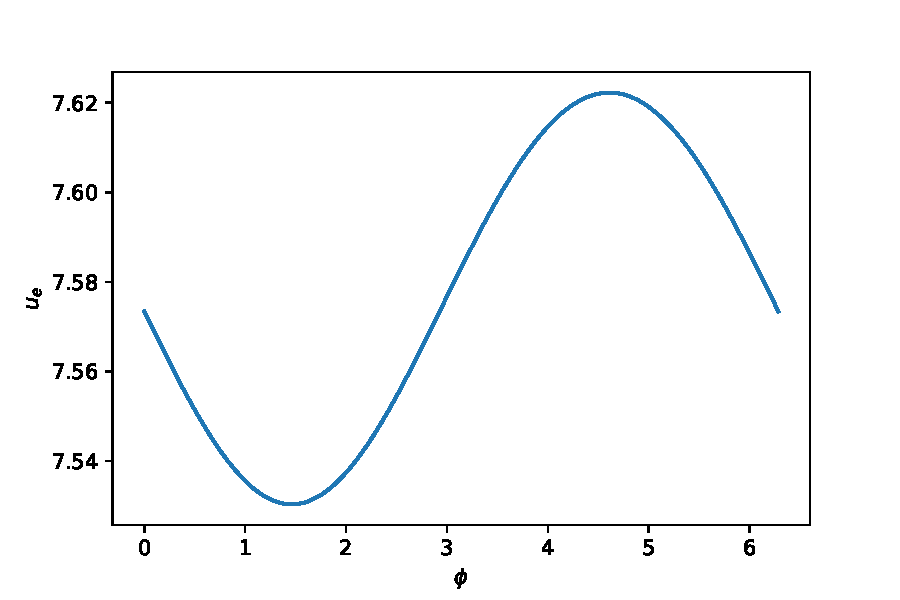
\includegraphics[width=\linewidth]{figures/NDA/Hotspot/phi1.pdf}  
\caption{The temperature required for a subcritical stockpile to ignite as we change the time of year the hotspot is introduced.}
\label{fig:hot:phi}
\end{figure} 

All of the results we have used to this stage rely on an ignition condition of $u_{\text{max}}=100$. We look at how this ignition criteria determines the critical temperature of the stockpile. For the range of ignition conditions we tested, $[10,100]$, the critical hotspot temperature did not change. This seems to suggest that setting a high enough temperature is sufficient for determining ignition in this simple model.\\ 

\begin{figure}[h!]
\centering
\begin{subfigure}{.5\textwidth}
  \centering
  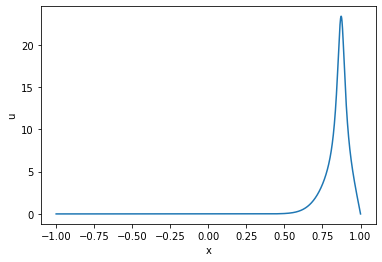
\includegraphics[width=\linewidth]{figures/NDA/Hotspot/Sample.png}  
  \caption{Stockpile after ignition}
  \label{fig:hot:ignited}
\end{subfigure}%
\begin{subfigure}{.5\textwidth}
  \centering
  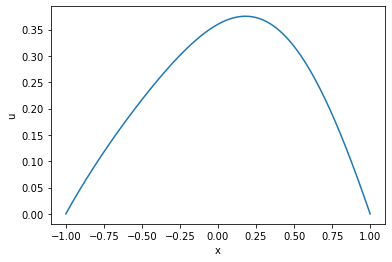
\includegraphics[width=\linewidth]{figures/NDA/Hotspot/Sample_sub.png}  
  \caption{Stockpile below critical hotspot}
  \label{fig:hot:sub}
\end{subfigure}
\caption{Temperature profiles within two identical stockpiles with different hotspot temperatures.}
\label{fig:hot:sample}
\end{figure}

Figure \ref{fig:hot:sample} compares a stockpile with nondimensional hotspot temperature, $u_h=7.53$, with a stockpile with $u_h=7.52$. This figure clearly indicates that it is the region of the hotspot itself, and the reactions occurring in that region which are causing the stockpiles to ignite. This provides further validation to the claim that as the ignition criteria is changed, the critical hotspot temperature remains the same. Figure \ref{fig:hot:sample} does then pose the question of what if the hotspot is inert. In the practical applications this hotspot could be material from a supercritical stockpile and the concentrations of the reactants can differ from those of a fresh subcritical stockpile. It may also be of value to know if we are able to put a region of heated material that does not react in order to promote combustion.\\

To investigate this behaviour we consider the extreme case of an inert material used in the hotspot region. In this region no reaction is occurring. We maintain the same assumptions as before regarding reactant consumption, that is we do not consider it.\\

\begin{figure}[h!]
\centering
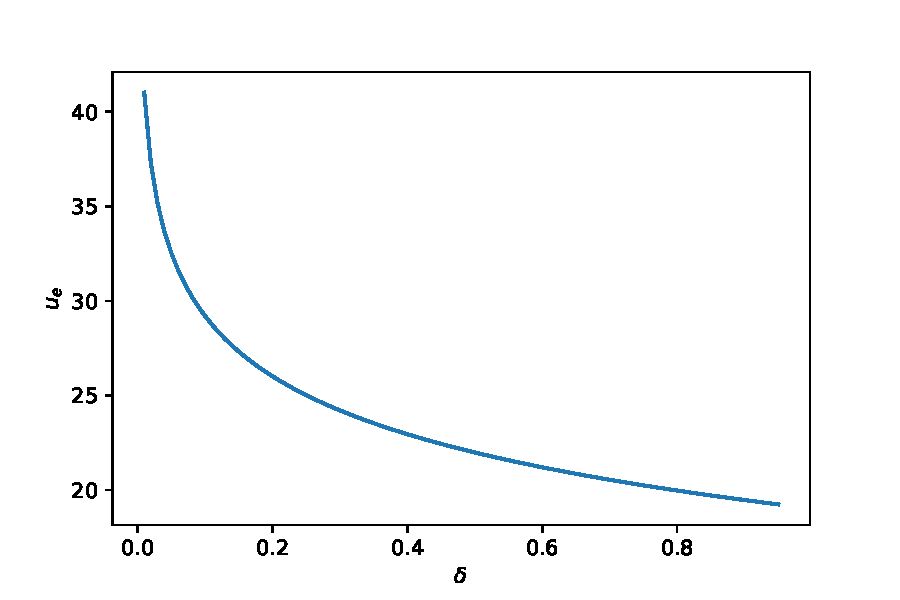
\includegraphics[width=\linewidth]{figures/NDA/Hotspot/delta_inert1.pdf}  
\caption{The temperature required for subcritical stockpile to ignite.}
\label{fig:hot:delta_inert}
\end{figure} 

Figure \ref{fig:hot:delta_inert} displays the same behaviour that we saw in Figure \ref{fig:hot:delta1} but we require a hotter hotspot in order to achieve ignition. This is intuitave as we need to heat the material surrounding the hotspot so that the material in those regions are heated. We can then compare the temperature profiles generated from identical stockpiles that have slightly different hotspot temperatures. 

\begin{figure}[h!]
\centering
\begin{subfigure}{.5\textwidth}
  \centering
  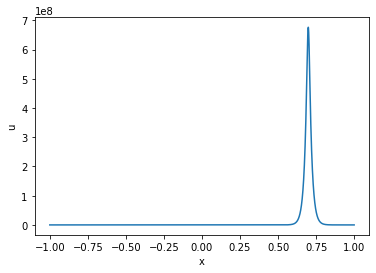
\includegraphics[width=\linewidth]{figures/NDA/Hotspot/Sample_inert.png}  
  \caption{Stockpile after ignition}
  \label{fig:hot:ignited_inert}
\end{subfigure}%
\begin{subfigure}{.5\textwidth}
  \centering
  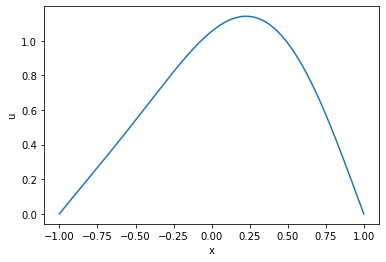
\includegraphics[width=\linewidth]{figures/NDA/Hotspot/Sample_sub_inert.png}  
  \caption{Stockpile below critical hotspot}
  \label{fig:hot:sub_inert}
\end{subfigure}
\caption{Temperature profiles within two identical stockpiles with different hotspot temperatures.}
\label{fig:hot:sample_inert}
\end{figure}

Figure \ref{fig:hot:sample_inert} displays these two sample temperature profiles. The temperature profiles are very similar to what we obtained when the hotspot reacted. The key difference is that in the ignited stockpiles the region where the stockpiles first ignite is adjacent to the hotspot rather than the spot itself. The difference in the non-dimensional hotspot temperatures of these two simulations is 0.0001, which for our parameters equates to roughly $0.0008^oC$. This is an extremely small difference for the results that we are observing. This implies that the critical values for the hotspot temperature are dependant upon the numerical solver and in this region, small pertubations in the initial condition can cause a large difference in the solution. Care needs to be taken when using the results in this region. This relatively small difference does highlight the need for consideration of the probability of our reaction parameters rather than using point values. This non-dimensional temperature is dependant upon the activation energy and thus any uncertainty in the activation energy will produce an uncertainty in this non-dimensional hotspot temperature. Considering the most efficient methonds in practice will be to minimise the temperature of the hotspot to cause ignition, knowledge of this uncertainty will be valueable.\\

Similarly, we can investigate the effect that location and size has on the hotspot. Figure \ref{fig:hot:size_loc_inert} display the various temperatures required. Figure \ref{fig:hot:loc_i} indicates that the bahaviour is very similar for inert hotspots and reactive hotspots as the location of the hotspot changes. When we change the size of the hotspot then the results become more interesting. If the hotspot is large then there are now reactions occurring inside the hotspot to generate additional heat. The smaller hotspots require higher temperatures as they inject less energy into the stockpiles. This leaves the two extreme cases to require high temperatures to induce ignition, leading to some minimum hotspot temperature being required. \\

\begin{figure}[h!]
\centering
\begin{subfigure}{.5\textwidth}
  \centering
  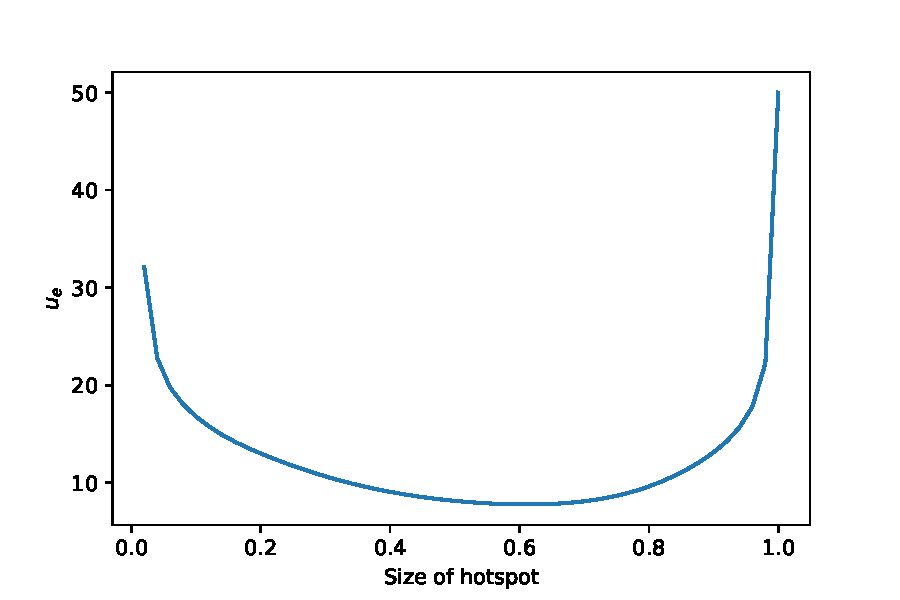
\includegraphics[width=\linewidth]{figures/NDA/Hotspot/size_inert1.pdf}  
  \caption{Hotspot temperature required for different size hotspots.}
  \label{fig:hot:size_i}
\end{subfigure}%
\begin{subfigure}{.5\textwidth}
  \centering
  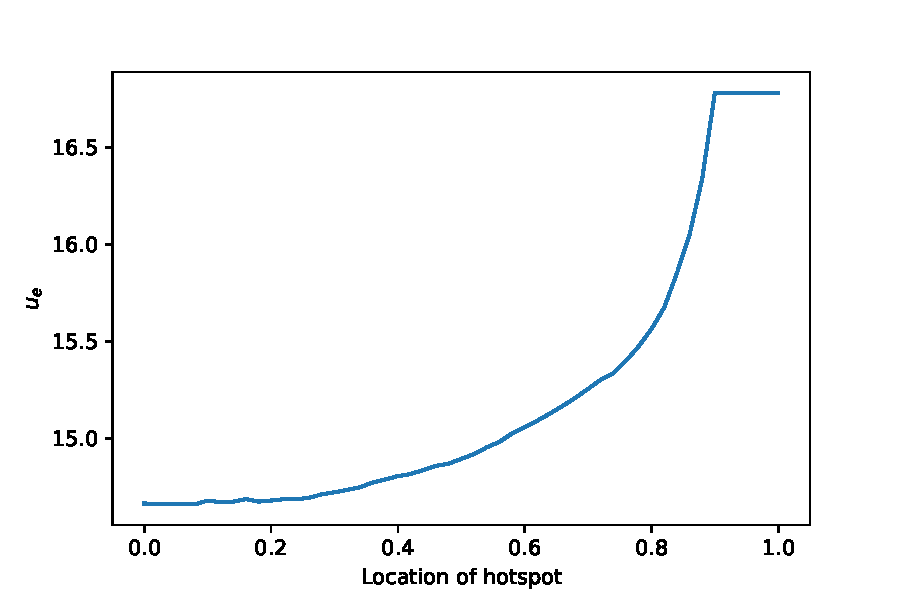
\includegraphics[width=\linewidth]{figures/NDA/Hotspot/Location_inert1.pdf}
  \caption{Hotspot temperature for different hotspot locations.}
  \label{fig:hot:loc_i}
\end{subfigure}
\label{fig:hot:size_loc_inert}
\caption{The critical hotspot temperature required to cause the ignition of subcritical stockpiles as the location and size of the hotspot vary.}
\end{figure}

Something that is worth considering if we seek to use larger hotspots is to account for the energy cost in heating heating the hotspot, and the logistics aspect of inserting this into the stockpile. Whilst some of the larger hotspots require a lower temperature to induce ignition, the cost of heating the increased amount of material can impact the optimal hotspot size.\\

The effect of periodic boundary conditions is similar to that or a reactive hotspot. There is an insignifcant difference though this is at the higher temperatures that are consistent with the inert stockpiles. We also observe the same behaviour when we change the ignition temperature. If we consider critical ignition temperatures that are too low, such that the critical hotspot temperature when $U_{\text{ig}}=100$, is greater than the ignition temperature then this results in subcritical stockpiles falsely identifying as having ignited.\\

 

